\documentclass{article}
%\usepackage[cyr]{aeguill}
\usepackage[utf8]{inputenc}
\usepackage[T1]{fontenc}
\usepackage[francais]{babel}
\usepackage{amsmath}
\usepackage{fancyhdr}
\usepackage{amsfonts}
\usepackage{makeidx}         
\title{Implémentation de l'algorithme du fast-marching pour la résolution d'un labyrinthe}
\usepackage[pdftex]{graphicx}
\author{Jean Prost \and Lucas Potin \and Edouard Gouteux}

\begin{document}
	
\maketitle
	
\section{L'algorithme du fast marching}

La méthode du fast marching a été introduite par James Setian. Cette méthode possède notamment des applications en mécanique des fluides et en traitement d'image. Cette méthode permet de résoudre l'équation d'Eikonal, de la forme :
\begin{equation}
|\nabla T|=\mathcal{F}
\end{equation}
Ici, $ \mathcal{F}$ et $T$ sont des fonctions $\mathbb{R}^n \to \mathbb{R}$, ou $n$ peut prendre la valeur 1, 2, où 3. $\mathcal{F}$ est la métrique donné du problème, et $T$ est la fonction à déterminer, avec comme condition initiale $T(x_0) = 0$. Ici nous nous concentrerons sur des fonctions $ \mathcal{F}$ et $T$ de $\mathbb{R}^2 \to \mathbb{R}$ :
\begin{equation}
|\nabla T(x,y)|=\mathcal{F}(x,y)
\end{equation}


\section{Programmation}

\section{Application à la recherche du plus court chemin dans un labyrinthe}
\subsection{Première approche}
On cherche à trouver le plus court chemin pour aller d'un point a à un point b dans un labyrinthe. Le labyrinthe nous est donné comme une image en noir blanc. Tout d'abord on normalise l'image : aux pixels blanc (où l'on peut passer) on affecte la valeur 1, aux pixels noir (que l'on ne peut pas franchir), on affecte la valeur 0. On construit ensuite notre métrique $W$ à partir de l'imager normalisé $I$, tel que pour tout pixel $ij$
\begin{equation}
W_{ij}  = \frac{1}{\epsilon+I_{ij}}
\end{equation}
Cette métrique pénalise donc les passages par les sommets infranchissables. La valeur$\epsilon$ au dénominateur permet d'éviter les divisions par zéro.
On applique ensuite l'algorithme du fast marchinq pour cette métrique, en choisissant comme point initiale l'entrée du labyrinthe. On obtient alors la fonction $T$ représentant la distance à notre sommet initial par rapport à la métrique W.

\begin{figure}[h]
	\begin{center}
		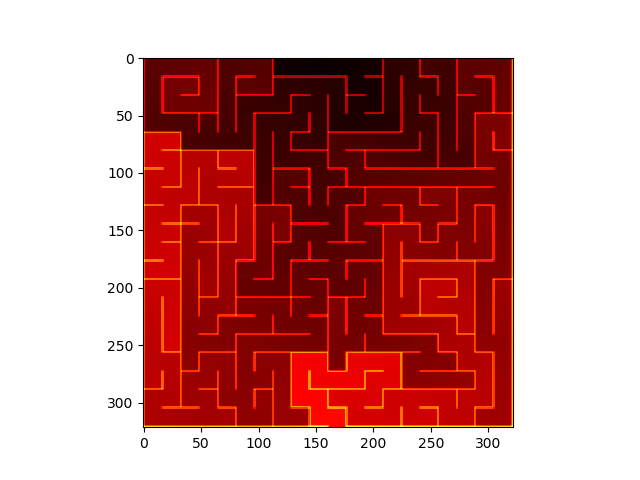
\includegraphics[scale=0.55]{../result/maze_T.png}
		\caption{distance au sommet initial (en haut au centre)}
	\end{center}
\end{figure}

On applique ensuite la descente du gradient sur la fonction T obtenue, en partant de l'autre extrémité du labyrinthe (celle que l'on n'a pas utilisé comme sommet initial). Le chemin nous est alors donné par les points obtenus au cours des itérations successives de la descente.

\begin{figure}[h]
	\begin{center}
		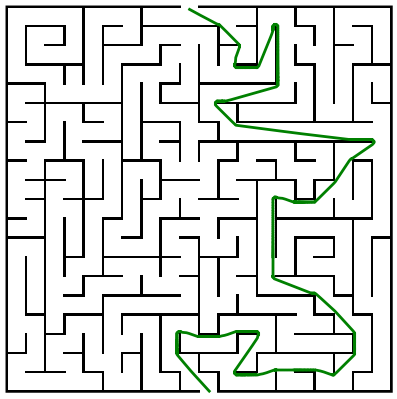
\includegraphics[scale=0.55]{../result/geo_maze.png}
		\caption{Solution du labyrinthe obtenue avec la descente du gradient}
	\end{center}
\end{figure}

\subsection{2 fois plus de fast marching!}
Le chemin obtenu est correcte, néanmoins il a tendance à "coller" les bords. Cela n'est pas très beau visuellement, et, pour certaines applications cela peut être problématique. Par exemple, dans le cas de la planification du chemin d'un robot, on peut souhaiter  que notre robot ne passe pas trop près des bords. Pour remédier à ce problème, une solution est d'inclure dans la métrique $W$ une pénalité pour les passages près des bords.

\end{document} 